% Template inspired by Drew Ulick
% https://www.overleaf.com/articles/130-cheat-sheet/ntwtkmpxmgrp
\documentclass{article}
\usepackage[landscape]{geometry}
\usepackage{xifthen}
\usepackage{url}
\usepackage{tikz}
\usetikzlibrary{positioning,fit,calc,backgrounds}

\usepackage{xcolor}
\usepackage{enumitem}
\usepackage{amssymb, amsmath,endnotes}
\usepackage{multicol}
\usepackage{multirow}
\usepackage{fontawesome}
\usepackage{xparse}
\usepackage[utf8]{inputenc}

\title{MISP Cheat Sheet}
\author{MISP Project}
\date{\today}

\makeatletter
\let\theauthor\@author
\let\thedate\@date
\makeatother
\advance\topmargin-.8in
\advance\textheight3in
\advance\textwidth3in
\advance\oddsidemargin-1.5in
\advance\evensidemargin-1.5in
\parindent0pt
\parskip2pt
\newcommand{\hr}{\centerline{\rule{3.5in}{1pt}}}
\newcommand{\events}{\texttt{Events }}
\newcommand{\event}{\texttt{Event }}
\newcommand{\attributes}{\texttt{Attributes }}
\newcommand{\attribute}{\texttt{Attribute }}
\newcommand{\objects}{\texttt{MISP Objects }}
\newcommand{\object}{\texttt{MISP Object }}
\newcommand{\reference}{\texttt{Reference }}
\newcommand{\references}{\texttt{References }}
\newcommand{\proposals}{\texttt{Proposals }}
\newcommand{\proposal}{\texttt{Proposal }}
\newcommand{\eventreports}{\texttt{Event Reports }}
\newcommand{\eventreport}{\texttt{Event Report }}
\newcommand{\sightings}{\texttt{Sightings }}
\newcommand{\sighting}{\texttt{Sighting }}
\newcommand{\taxonomies}{\texttt{Taxonomies }}
\newcommand{\taxonomy}{\texttt{Taxonomy }}
\newcommand{\galaxy}{\texttt{Galaxy }}
\newcommand{\galaxies}{\texttt{Galaxies }}
\newcommand{\clusters}{\texttt{Galaxy Clusters }}
\newcommand{\cluster}{\texttt{Galaxy Cluster }}
\newcommand{\sharinggroups}{\texttt{Sharing Groups }}
\newcommand{\sharinggroup}{\texttt{Sharing Group }}

\newcommand{\taggable}{\faicon{tags}\hspace*{0.3em}}
\newcommand{\distributable}{\faicon{eye-slash}\hspace*{0.3em}}
\newcommand{\synchronisable}{\faicon{exchange}\hspace*{0.3em}}
%\colorbox[HTML]{e4e4e4}{\makebox[\textwidth-2\fboxsep][l]{texto}
\tikzstyle{mybox} = [
    draw=black,
    fill=white,
    very thick,
    rectangle, rounded corners,
    inner sep=10pt, inner ysep=10pt
]
\tikzstyle{boxtitle} = [
    % fill=white,
    % draw=black,
    % text=black,
    fill=black,
    text=white,
    font=\bfseries,
    right=10pt
]
% arg1 = icon
% arg2 = purpose
% arg3 = usecase
% arg4 = actions
% arg5 = description
% arg6 = title
% arg7 = content
\tikzset{actionbox/.style={
    text=white,
    yshift=-1pt,xshift=-1pt,
    append after command={
    \pgfextra
            \draw[sharp corners, fill=black]% 
        (\tikzlastnode.west)% 
        [rounded corners=0pt] |- (\tikzlastnode.north)% 
        [rounded corners] -| (\tikzlastnode.east)% 
        [rounded corners=0pt] |- (\tikzlastnode.south)% 
        [rounded corners] -| (\tikzlastnode.west);
    \endpgfextra
    }
}}
\NewDocumentCommand{\cheatbox}{ O{} O{} O{} O{} O{} m m}{
    \begin{tikzpicture}
        \node [mybox] (box){%
            \begin{minipage}{0.3\textwidth}
            \ifthenelse{\isempty{#4}}{}{\vspace{1em}}
            \textit{#5}
            \vspace*{0.3em}
            \ifthenelse{\isempty{#2}}{}{ \par{\textbf{Purpose}: #2}}
            \ifthenelse{\isempty{#3}}{}{ \par{\textbf{Usecase}: #3\\}}
            #7
            \end{minipage}
        };
        \node[boxtitle] at (box.north west) {#1 #6};
        \ifthenelse{\isempty{#4}}{}{
            \path node [actionbox, anchor=north east] at (box.north east) (actionLabel) {#4};
        }
    \end{tikzpicture}

    \vspace*{2pt}
}
% arg1 = description
% arg2 = title
% arg3 = content
\newcommand{\cheatboxlarge}[3][]{
    \begin{tikzpicture}
        \node [mybox] (box){%
            \begin{minipage}{0.46\textwidth}
            \textit{#1}
            \ifthenelse{\isempty{#1}}{}{\vspace{2pt}}
            #3
            \end{minipage}
        };
        \node[boxtitle] at (box.north west) {#2};
    \end{tikzpicture}

    \vspace*{4pt}
}
% arg1 = label
% arg2 = text
\newcommand{\boxentry}[2]{
    \par{\textbf{#1}: #2\vspace*{0.3em}}
}
% arg1 = label
% arg2 = text
\newcommand{\boxentrycompact}[2]{
    \par{\textbf{#1} #2}
}

% arg1 = current level
% arg2 = text
\newcommand{\changestyledistribution}[2]{
    % \ifthenelse{\isin{#1}{#2}}{
    \ifthenelse{#1 > #2}{
        \tikzset{currentstyle/.style=fullnode}
    }{
        \tikzset{currentstyle/.style=emptynode}
    }
}
% arg1 = label
% arg2 = text
\newcommand{\distrigraph}[1]{
    \def \scale {0.2}
    \begin{tikzpicture}[
        emptynode/.style={circle, draw=black, scale=\scale},
        fullnode/.style={circle, draw=black, fill=black, scale=\scale},
    ]
    \tikzset{
        currentstyle/.style={}
    }
        \changestyledistribution{#1}{0}
        \node[currentstyle] (d0)  {};
        \changestyledistribution{#1}{1}
        \node[currentstyle] (d1a) [above right= 1pt and 30pt of d0] {};
        \node[currentstyle] (d1b) [below right= 1pt and 30pt of d0] {};
        \changestyledistribution{#1}{2}
        \node[currentstyle]  (d2)  [right=of d1b] {};
        \changestyledistribution{#1}{2}
        \node[currentstyle]  (d3)  [right=of d2] {};

        \draw[-] (d0) to[out=30, in=180] (d1a);
        \draw[-] (d0) to[out=-30, in=180] (d1b);
        \draw[-] (d1b) -- (d2);
        \draw[-] (d2) -- (d3);
    \end{tikzpicture}
}

\begin{document}

\begin{center}{
    \huge{\textbf{MISP Concept Cheat sheet}}}\\
\end{center}
\begin{multicols*}{2}

% \cheatboxlarge{Legend}{
%     \boxentry{\faicon{tags}}{Context can be attached to the element}
%     \boxentry{\faicon{lowVision}}{Can have a distribution level}
%     \boxentry{\faicon{exchange}}{Can be synchronised to other instances}
%     \boxentry{$\blacklozenge \owns \blacktriangle$}{The element $\blacklozenge$ can act as a container and contains $\blacktriangle$}
% }
\cheatboxlarge{Glossary}{

    \boxentry{Correlations}{Are created automatically when an \attribute is created or modified. It links two \events having values that matches according to the correlation engine}
    \boxentry{Correlation Engine}{Is the system used by MISP to create correlation between \attribute's value. It currently support strict string comparison, SSDEEP and CDIR blocks matches.}
    \boxentry{Caching}{Is the process of \textit{pulling} data from another MISP instance or a feed but only storing hashes of the collected values to be used for correlations.}
    \boxentry{Delegation}{Is the act of delegating the publication and the ownership of an \event to another organisation, thus hiding the original creator of the \event.}
    \boxentry{Deletion (soft)}{Is the act flagging an element as deleted and thus propagating the revocation among the network of connected MISP instances.}
    \boxentry{Deletion (hard)}{Is the act of removing the element from the database. It will thus do not perform revocation on other MISP instances.}
    \boxentry{Extended \event}{Is an \event that extends an existing \event, providing a combined view of the data contained in both \events. The owner of the extending \event is the organisation that created the extension, this allowing anyone to extend any \events and altering those.}
    \boxentry{\galaxy Matrix}{Is a matrix derived from \clusters belonging to the same \galaxy. The layout (pages and columns) is defined at the \galaxy level while its content comes from the \clusters themselves.}
    \boxentry{IoC}{And Indicator Of Compromise is an \attribute having the \texttt{to\_ids} flag set}
    \boxentry{Publishing}{For an \event or a \cluster to be synchronised, they must be \textit{published}. \textit{publishing} an \event will also send e-mail notifications and expose it to certain format requiring the \event to be in this state.}
    \boxentry{Pulling}{Is the process of using the configured sync user on a remote instance to fetch the accessible data and store it.}
    \boxentry{Pushing}{Is the process of using the configured uplink connection to send data to a remote instance.}
    \boxentry{Synchronisation}{Is the exchange of data between two (or more) MISP instances throught the \textit{pull} and \textit{push} mechanism.}
    \boxentry{Sync. filtering rule}{Rules that can be applied on a synchronisation link for both the \textit{pull} and \textit{push} mechanism allowing to block the data matching or not said rule.}
    \boxentry{Sync. User}{Special role of a user granting addional sync permissions. The recommanded way to setup \textit{pull} and \textit{push} synchronisation is to use \textit{sync users}.}
    \boxentry{Proposals}{Are a mechanism to propose modications to the creating organisations. If a path of connected MISP instances exists, it will be synchronized so that the creator may accept or discard it.}
}

\columnbreak
\cheatboxlarge[Controls who can see the data and how it should be synchronised.]{Distribution}{
    \boxentry{Organisation only}{Only members of your organisation}
    \boxentry{This community}{Organisations on this MISP instance}
    \boxentry{Connected Communities}{Organisations on this MISP instance and those on MISP instances synchronising with this one. Upon receiving data, the distribution level will be downgraded to \texttt{This community} to avoid further propagation.}
    \begin{center}\distrigraph{2}\end{center}
    \boxentry{All Communities}{Anyone having access: Will be freely propagated in the network of connected MISP instances.}
    \begin{center}\distrigraph{3}\end{center}
    \boxentry{Sharing Groups}{Organisations being part of the distribution list that exhaustively keeps track of who can access the data and how it should be synchronised.}

    \begin{multicols*}{2}
    \begin{center}
        \begin{tabular}{| l | l |}
            \hline
            \multicolumn{2}{|c|}{\sharinggroup configuration} \\
            \hline
            \multirow{3}{*}{Organisations} & Org. $\alpha$\\
                & Org. $\omega$\\
                & Org. $\gamma$\\
            \hline
            \multirow{3}{*}{Instances*} & MISP 1\\
                & MISP 2\\
                & MISP 3\\
            \hline
        \end{tabular}\\
        \hspace*{-2em}*Or enable roaming mode
    \end{center}
    \columnbreak

    \begin{center}
    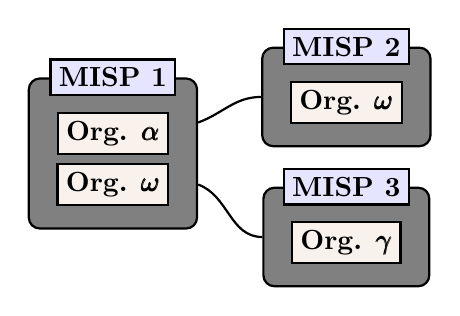
\begin{tikzpicture}[
        node/.style={inner sep=0pt},
        simplebox/.style n args={3}{
            rectangle, rounded corners, thick,
            draw=black, fill=#1,
            minimum width=#2,
            minimum height=#3,
            inner sep=10pt, inner ysep=10pt
        },
        simpleboxtitle/.style = {
            rectangle, rounded corners=0,
            minimum width=1em,
            fill=brown!10, text=black, draw, thick,
            font=\bfseries,
            inner sep=3pt
        },
        header/.style = {%
            inner ysep = +1.0em,
            append after command = {
                \pgfextra{\let\TikZlastnode\tikzlastnode}
                node[simpleboxtitle] (header-\TikZlastnode) at (\TikZlastnode.north) {#1}
            }
        },
        coloredHeader/.style n args={2}{
            inner ysep = +1.0em,
            append after command = {
                \pgfextra{\let\TikZlastnode\tikzlastnode}
                node[simpleboxtitle,fill=#2] (header-\TikZlastnode) at (\TikZlastnode.north) {#1}
            }
        }
    ]

        \node[simpleboxtitle] (orgs01) [] {Org. $\pmb{\alpha}$};
        \node[simpleboxtitle] (orgs02) [below = 0.3em of orgs01] {Org. $\pmb{\omega}$};
        \node[fit = (orgs01) (orgs02)] (orgs0) {};
        \node[simpleboxtitle] (orgs1) [above right= -0.8em and 4em of orgs0] {Org. $\pmb{\omega}$};
        \node[simpleboxtitle] (orgs2) [below = 3.5em of orgs1] {Org. $\pmb{\gamma}$};
        \begin{scope}[on background layer]
            \node[yshift=2pt, fit = (orgs01) (orgs02), simplebox={gray}{1em}{2em}, coloredHeader={MISP 1}{blue!10}] (m1) {};
            \node[yshift=2pt, fit = (orgs1), simplebox={gray}{1em}{2em}, coloredHeader={MISP 2}{blue!10}] (m2) {};
            \node[yshift=2pt, fit = (orgs2), simplebox={gray}{1em}{2em},  coloredHeader={MISP 3}{blue!10}] (m3) {};
        \end{scope}

        \draw[-, thick] (m1) to[out=20, in=180] (m2);
        \draw[-, thick] (m1) to[out=-20, in=180] (m3);
    \end{tikzpicture}
    \end{center}
    \end{multicols*}
}
\cheatboxlarge[The act of \textbf{sharing} where everyone can be a consumer and/or a producer.]{Synchronisation}{

    \vspace*{0.3em}
    A one way synchronisation link between two MISP instances. Organisation $\alpha$ created a \textit{sync user} \faicon{user-plus} on MISP 2 and noted down the generated API Key. A synchronisation link can be created on MISP 1 using the API Key and the organisation of the \textit{sync user}. At that point, MISP 1 can \textit{pull} data from MISP 2 and \textit{push} data to MISP 2.

    \begin{center}
    \pgfdeclarelayer{bg0}    % declare background layer
    \pgfdeclarelayer{bg1}    % declare background layer
    \pgfsetlayers{bg0,bg1,main}  % set the order of the layers (main is the standard layer)
    \begin{tikzpicture}[
        simplebox/.style n args={3}{
            rectangle, rounded corners, thick,
            draw=black, fill=#1,
            minimum width=#2,
            minimum height=#3,
            inner sep=10pt, inner ysep=10pt
        },
        simpleboxtitle/.style = {
            rectangle, rounded corners=0,
            minimum width=1em,
            fill=brown!10, text=black, draw, thick,
            font=\bfseries,
            inner sep=3pt
        },
        header/.style = {%
            inner ysep = +1.0em,
            append after command = {
                \pgfextra{\let\TikZlastnode\tikzlastnode}
                node[simpleboxtitle] (header-\TikZlastnode) at (\TikZlastnode.north) {#1}
            }
        },
        coloredHeader/.style n args={2}{
            inner ysep = +1.0em,
            append after command = {
                \pgfextra{\let\TikZlastnode\tikzlastnode}
                node[simpleboxtitle,fill=#2] (header-\TikZlastnode) at (\TikZlastnode.north) {#1}
            }
        },
        user/.style = {
            inner sep=0pt
        },
        legend/.style = {
            rectangle, rounded corners=0,
            inner sep=2pt,
            draw=black
        },
        nodes = {align = center}
    ]

        \node[user] (misp1users) {\faicon{user} \faicon{user} \faicon{user}};
        \node[user] (misp2users) [right= 13em of misp1users] {\faicon{user} \faicon{user}};
        \node[user] (misp2users2) [right= 3em of misp2users] {\faicon{user} \faicon{user} \faicon{user}};
        \node[user,inner xsep=3pt] (syncuser) [left= 0.0em of misp2users] {\faicon{user-plus}};
        \begin{pgfonlayer}{bg1}
            \node[yshift=2pt, fit = (misp1users), simplebox={white}{1em}{2em}, header = Org. $\pmb{\alpha}$] (misp1org) {};
            \node[yshift=2pt, fit = (misp2users) (syncuser), simplebox={white}{1em}{2em}, header = Org. $\pmb{\alpha}$] (misp2org) {};
            \node[yshift=2pt, fit = (misp2users2), simplebox={gray!30}{1em}{2em}, header = Org. $\pmb{\omega}$] (misp2org2) {};
        \end{pgfonlayer}
        \begin{pgfonlayer}{bg0}
            \node[yshift=+0.5em, fit = (misp1org), simplebox={gray}{11em}{6em}, coloredHeader={MISP 1}{blue!10}] (m1) {};
            \node[yshift=+0.5em, fit = (misp2org) (misp2org2), simplebox={gray}{11em}{6em}, coloredHeader={MISP 2}{blue!10}] (m2) {};
        \end{pgfonlayer}
        \draw[-,very thick] (m1.south) -- ++(0,-15pt) -| ($(syncuser.south) + (0,-2pt)$) node [
            pos=0.25,above,yshift=-0.9em
        ] (textsync) {Sync. connection};
        \def \offsetY {3}
        \draw[->,thick] ($(m1.east) + (1pt,\offsetY pt)$) -- ($(m2.west) + (-1pt,\offsetY pt)$) node [above,midway,yshift=-\offsetY pt] {PUSH};
        \draw[<-,thick] ($(m1.east) + (1pt,-\offsetY pt)$) -- ($(m2.west) + (-1pt,-\offsetY pt)$) node [below,midway,yshift=\offsetY pt] {PULL};
    \end{tikzpicture}
    \end{center}
}
\end{multicols*}
\newpage

\begin{center}{
    \huge{\textbf{MISP Data Model Cheat Sheet}}}\\
\end{center}
\begin{multicols*}{3}
    \cheatbox{Legend}{
        \boxentrycompact{\taggable}{Context such as \taxonomies or \clusters can be attached to the element}
        \boxentrycompact{\distributable}{Can have a distribution level}
        \boxentrycompact{\synchronisable}{Can be synchronised to other instances}
        % \boxentry{$\blacklozenge \owns \blacktriangle$}{The element $\blacklozenge$ can act as a container and contains $\blacktriangle$}
    }

    % EVENT 
    \cheatbox[\faicon{user}]
        [Group datapoints and contexts together. Acting as an envelop, it allows setting its distribution and sharing rules.]
        [Encode incidents, events, reports, …]
        [\taggable \distributable \synchronisable]
        [Encapsulations for contextually linked information.]
        {Event}
        {
            $\blacktriangleright$ \events can contain other elements such as \attributes, \objects and \eventreports.
        }

    % ATTRIBUTE 
    \cheatbox[\faicon{cube}]
        [Individual data point. Can be an indicator or supporting data.]
        [Domain, IP, link, sha1, attachment, …]
        [\taggable \distributable \synchronisable]
        [Basic building block to share information.]
        {Attribute}
        {
            $\blacktriangleright$ \attributes cannot be duplicated inside the same \event and can have \sightings.
        }

    % Object 
    \cheatbox[\faicon{cubes}]
        [Groups \attributes that are intrinsically linked together.]
        [File, person, credit card, x509, device, …]
        [\distributable \synchronisable]
        [Advanced building block providing \attribute compositions via templates.]
        {MISP Object}
        {
            $\blacktriangleright$ \objects have their formats described in their respective template. They contain \attributes and can reference \reference other \attributes or \objects.
        }
    \columnbreak

    % Object Reference
    \cheatbox[$\nearrow$]
        [Allows to create relationships between entities, thus creating a graph where they are the edges and entities are the nodes]
        [Represent behaviours, similarities, affiliation, …]
        [\synchronisable]
        [Relationships between individual building blocks.]
        {Object Reference}
        {
            $\blacktriangleright$ \references can have a textual relationship which can come from MISP or be set freely.
        }

    % Sightings
    \cheatbox[\faicon{eye}]
        [Allows to add temporality to the data]
        [Record activity or occurence, perform IoC expiration, …]
        [\synchronisable]
        [Means to convey that a data point has been seen.]
        {Sightings}
        {
            $\blacktriangleright$ \sightings are the best way to express that something has been seen. They can also be used to mark \textit{false positives}.
        }

    % Event report
    \cheatbox[\faicon{file-text}]
        [Supporting data point to describe events or processes]
        [Encode reports, provide more information about the \event, …]
        [\distributable \synchronisable]
        [Advanced building block that can contain text.]
        {Event Report}
        {
            $\blacktriangleright$ \eventreports are markdown-aware and includes a special syntax to reference data points or context.
        }

    % Proposals
    \cheatbox[\faicon{comment}]
        [Allow the correction or the creation of \attributes for \events your organisation does not own.]
        [Disable the IDS flag, Correct errors]
        [\synchronisable]
        [Clone of an \attribute containing information about modification to be done.]
        {Proposals}
        {
            $\blacktriangleright$ As \proposals are sync., if the creator organisation is connected to the MISP instance from where the \proposal has been created, it will be able to either \textit{accept} or \textit{discard} it. 
        }

\end{multicols*}
\end{document}
